\begin{figure}[!htb]
	\centering

	\begin{tikzpicture}

		\node (Before) at (0,0) {
			\begin{tikzpicture}[scale=0.15]
				\coordinate (1) at (-5,-8);
				\coordinate (2) at (10,2);
				\coordinate (3) at (10,10);
				\coordinate (4) at (-7,1);
				\coordinate (5) at (-1,8);
				\coordinate (6) at (-4,-9);
				\coordinate (7) at (5,-3);
				\coordinate (8) at (6,4);
				\coordinate (9) at (3,-5);
				\coordinate (10) at (0,1);

				\draw[thick, blue] (2) -- (10);
				\draw[thick, blue] (1) -- (4);
				\draw[thick, blue] (4) -- (5);

				\foreach \i in {1, ..., 10}{
						\filldraw[black] (\i) circle (4pt);
					}
			\end{tikzpicture}
		};

		\node (Delaunay) at (6,0) {
			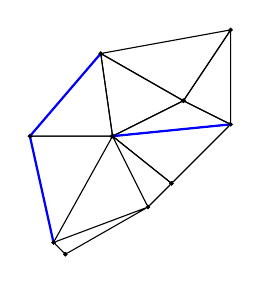
\begin{tikzpicture}[scale=0.15]
				\coordinate (1) at (-5,-8);
				\coordinate (2) at (10,2);
				\coordinate (3) at (10,10);
				\coordinate (4) at (-7,1);
				\coordinate (5) at (-1,8);
				\coordinate (6) at (-4,-9);
				\coordinate (7) at (5,-3);
				\coordinate (8) at (6,4);
				\coordinate (9) at (3,-5);
				\coordinate (10) at (0,1);

				\draw[rounded corners=1pt] (4) -- (5) -- (10) -- cycle;
				\draw[rounded corners=1pt] (1) -- (6) -- (9) -- cycle;
				\draw[rounded corners=1pt] (5) -- (8) -- (10) -- cycle;
				\draw[rounded corners=1pt] (2) -- (8) -- (10) -- cycle;
				\draw[rounded corners=1pt] (7) -- (9) -- (10) -- cycle;
				\draw[rounded corners=1pt] (2) -- (7) -- (10) -- cycle;
				\draw[rounded corners=1pt] (3) -- (5) -- (8) -- cycle;
				\draw[rounded corners=1pt] (2) -- (3) -- (8) -- cycle;
				\draw[rounded corners=1pt] (1) -- (4) -- (10) -- cycle;

				\draw[thick, blue] (2) -- (10);
				\draw[thick, blue] (1) -- (4);
				\draw[thick, blue] (4) -- (5);

				\foreach \i in {1, ..., 10}{
						\filldraw[black] (\i) circle (4pt);
					}
			\end{tikzpicture}
		};

		% % Arrow between them
		\draw[->, thick] (Before.east) -- (Delaunay.west);

	\end{tikzpicture}

	\caption{Edge constraints for Delaunay triangulation}\label{fig:constrainedDelaunay}
\end{figure}

